%\documentclass[twocolumn, trackchanges]{aastex6}
\documentclass[preprint2]{aastex62}


\bibliographystyle{aasjournal}
\usepackage{graphicx}
\usepackage[suffix=]{epstopdf}
\usepackage{natbib}
\usepackage{amsmath}
\usepackage{url}
\usepackage{xspace}



%    Make Scientific Notation
\providecommand{\e}[1]{\ensuremath{\times 10^{#1}}}

% make the word Kepler italicized, deal w/ floating space afterwards
\newcommand{\Kepler}{\textsl{Kepler}\xspace}

\begin{document}

%%%%%%%%%%%%%%%%%%%%%%
\title{Searching for Active Latitudes Using Transiting Exoplanets}

\shorttitle{Starspot Latitudes}
\shortauthors{Davenport et al.}


\author{James. R. A. Davenport}
%\altaffiliation{NSF Astronomy and Astrophysics Postdoctoral Fellow; DIRAC Fellow}
\altaffiliation{DIRAC Fellow}
\affiliation{Department of Astronomy, University of Washington, Seattle, WA 98195, USA}

\author{Brett M. Morris}
\affiliation{Department of Astronomy, University of Washington, Seattle, WA 98195, USA}

\author{Leslie Hebb}
\affiliation{Department of Physics, Hobart and William Smith Colleges, Geneva, NY, 14456}

\author{Michelle Gomez}
\affiliation{Department of Physics, Hobart and William Smith Colleges, Geneva, NY, 14456}

\author{Eric Agol}
\affiliation{Department of Astronomy, University of Washington, Seattle, WA 98195, USA}

\author{Suzanne L. Hawley}
\affiliation{Department of Astronomy, University of Washington, Seattle, WA 98195, USA}



%%%%%%%%%%%%%%%%%%%%%%%%%%%%%%
\begin{abstract}
Active latitude bands, as well as the ``Solar Butterfly Diagram'', are foundational properties that drive models of the solar dynamo. However, while considerable progress has been made on modeling stellar dynamos, no comparable constraint for the latitude distribution of active regions has been available. Here we present an ensemble approach to studying the latitude distribution of starspots using \Kepler transiting exoplanets. By exploiting the differences in impact parameter ($b$), the planets occult a range of latitude bands. We find X, using Y stars, and note Z. The future is bright.
\end{abstract}

\keywords{stars: activity}


%%%%%%%%%%%%%%%%%%%%%%%%%%%%%%
\section{Introduction}
\label{sec:intro}

The latitude range over which sunspots form throughout the course of the solar activity cycle is a key observable constraint in stellar dynamo theory. 
Spots trace the local surface magnetic field, and are therefore valuable for understanding the geometry and strength of a star's internal magnetic field \citep{berdyugina2005}.
For the Sun, spots predominantly form within two roughly symmetric bands of latitude centered about the equator. Throughout the $\sim$11 year solar activity cycle, the mean latitudes of these bands decreases towards the equator, from $\sim$$30^\circ$ to $\sim$$5^\circ$ \citep[e.g. see][]{babcock1961}. This sunspot latitude variation over time is known as the ``Sp\"{o}rer's Law'' (or colloquially as the Butterfly diagram), and was first summarized by \citet{maunder1904}.

``Active latitudes'' as observed on the Sun occur naturally as a result of both stellar rotation and differential rotation, which together govern the activity cycle length in the $\alpha\Omega$ mean-field dynamo model \citep{brandenburg2005}. The rate of stellar mass and angular momentum loss over time is also dependent on the surface magnetic field morphology \citep{garraffo2015}, and improvements in stellar spin-down models will require advances in surface magnetic field maps \citep{garraffo2016}.
Determining the latitudes of starspots is therefore vital for calibrating mean field dynamo theory from the Sun to other stars.



Much work has been done to search for other observable constraints of Solar-like dynamo activity in other stars.
Considerable effort has been made to search for overall magnetic activity cycles for stars, primarily in measuring chromospheric Ca II H\&K emission over many decades \citep[e.g.]{wilson1978,baliunas1995}. These surveys require long observation baselines, and have yielded many potential activity cycle detections from samples of hundreds of nearby stars. Starspot-modulation rotation curves have been measured for tens of thousands of stars using space-based photometric monitoring \citep{mcquillan2014}, providing evidence of stellar dynamos producing surface spots. Differential rotation constraints using starspot modulation curves has been attempted \citep[e.g.][]{reinhold2013}, but remains effectively unconstrained due to degeneracies between spot evolution and differential rotation\citep{aigrain2015}. A few notable exceptions have been found for rapidly rotating stars with slowly evolving, long-lived spots \citep[e.g.][]{morin2008a,davenport2015b}, but these are likely due to polar starspots that represent non-Solar dynamo type activity. 


Despite its importance, starspot latitudes have only been constrained for a handful of systems. %-- a natural result of stellar surfaces being unresolved due to their great distance. 
Coarse maps of the stellar magnetic field can be generated via Doppler Imaging techniques for rapidly rotating stars \citep{semel1989,donati_brown1997}, but typically cannot resolve small enough size scales to study individual spots comparable to those observed on the Sun.
For a small number of nearby active stars, the surface can be imaged directly via interferometry. \cite{roettenbacher2016} made use of this method to map the starspots on the old active star, $\zeta$ And, finding no sign of a solar-like spot distribution. Techniques for constraining starspot latitudes for larger samples of stars, particularly for older or slower rotating stars, are desperately needed.


Here we introduce a statistical approach to mapping the distribution of starspots as a function of stellar latitude for stars with a transiting exoplanet. Transiting exoplanets have been previously used to probe the starspot activity along single latitude bands for individual stars \citep[e.g.][]{morris2017}. By exploiting the varying geometry for many transiting systems, specifically the impact parameter, we seek to create an ensemble portrait of the latitudes where starspots are most prevalent. While the detailed geometry of each transiting planet+star system requires careful consideration to correctly map observed features back to precise stellar latitudes, the method can in principle be applied to characterize a great number of transit host stars. This approach can be extended beyond single-band transit photometry, which will help measure detailed active region properties, and with extended monitoring campaigns of transits we may be able to simultaneously model the stellar activity cycles.



%%%%%%%%%%%%%%%%%%%%%%
\section{Starspot Properties from Transit Tomography}
\label{sec:transit}

Transiting exoplanets provide a unique means to trace small-scale features on the surface of stars. As the planet passes in front of its host star, varying intensities of flux on the stellar surface due to hot or cool regions change the transit depth. In this ``transit tomography'', the planet provides a one-dimensional map of the surface brightness. When the planet passes over cool starspots, the transit depth is briefly {\it shallower}, resulting in ``bumps'' in the transit light curve \citep{silva2003}. The measured amplitude of these bumps are determined by the planet size relative to the star (which governs the overall transit depth), the starspot size relative to the planet, and the temperature contrast of the spot to the average photosphere. For bright, nearby stars with transiting Neptune or Jupiter sized planets, these bumps can reach $\sim$1/4 the transit depth.

The most informative scenario for constraining the latitude distribution of starspots occurs when the stellar rotation and planetary orbital axes are significantly misaligned \citep{llama2012}, as is the case for Hat-P-11 \citep{sanchis-ojeda2011}. In this geometry, the planet passes in front of the star in a nearly orthogonal direction to the rotation axis, mapping out a range of latitudes with each transit along a nearly constant line of stellar longitude. For Hat-P-11, two distinct active latitude bands have been discovered, which reveal a solar-like dynamo at work \citep{morris2017}. However, for most transiting systems the planetary orbit and stellar spin axes are well aligned, resulting in a fixed range of latitudes sampled by every transit, as in the Kepler 17 system \citep{davenport_phd}. While long term monitoring of these transiting systems allows us to track starspot evolution, the global spot distribution cannot be probed. Transiting multi-planet systems may provide another means to study a range of latitudes for a single star \citep[e.g. Kepler 186; ][]{kepler186f}, but the sample of such systems is currently quite small.


%%%%%
\begin{figure}[!t]
\centering
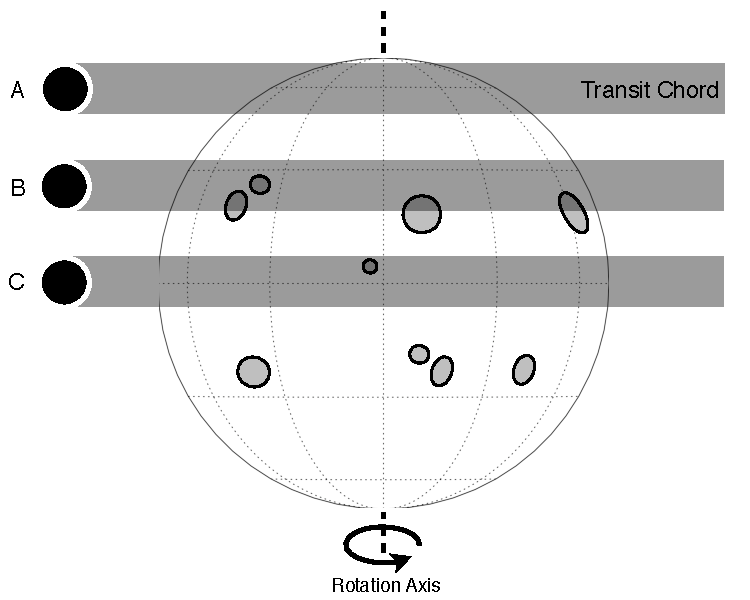
\includegraphics[width=3.5in]{diagram1}
\caption{
Schematic diagram of star with active starspot latitudes centered at $\sim$25$^\circ$ latitude, and three transiting exoplanets with impact parameters ranging between nearly b=1 (A) to  b=0 (C). The planet size is typical of a hot Jupiter, with $r_p/r_\star\approx 0.11$.
}
\label{fig:diagram1}
\end{figure}


Naturally, to detect a starspot bump in transit the transit chord as projected onto the star must intersect regions on the surface containing starspots. In Figure \ref{fig:diagram1} we demonstrate three identical transiting exoplanets with differing impact parameters, whose transits project onto different ranges in latitude on the star. The starspots are placed at typical latitudes for those found on the Sun, here centered at $\sim$25$^\circ$ latitude. In this case, the intermediate transit (planet B) with an impact factor of $b=0.5$ intersects the northern active latitude of the star. 
POINT: WE CAN USE IMPACT PARAMETER TO PROBE LATITUDE




Missions like \Kepler now routinely observe transits with the photometric precision required to detect these bumps \citep{borucki2010}, and indeed many \Kepler systems have had their spot properties measured from this technique \citep[e.g.][]{sanchis-ojeda2011, sanchis-ojeda2013}. In the best cases, for bright stars and with 1-minute cadence, hundreds of individual starspots have been detected \citep[e.g.][]{davenport_phd}, and fit with detailed forwarding modeling (Hebb et al. in prep). However, many transiting systems in \Kepler are either too faint, or have too slow of an observing cadence (e.g. the \Kepler 30-minute cadence), to resolve individual starspot bumps. Transits from these fainter stars may still be impacted by starspot crossing events, with transit depths or durations appearing to vary due to changing numbers of starspots on the observable surface.



As we combine lots of transits, we get lots of scatter in vs out of transit!
show example from Kepler17
POINT: WE CAN USE ENSEMBLE OF POORLY RESOLVED TRANSITS TO QUANTIFY SPOTTEDNESS


%%%%%
\begin{figure}[!t]
\centering
\includegraphics[width=3.5in]{kepler17_alltransits_old}
\caption{
Overlay of every short-cadence \Kepler transit for Kepler 17 from \citet{davenport_phd}. Starspot variations have been normalized out using second-order polynomial fits to the out-of-transit regions. The binned median (solid line) and standard deviation (dashed line) show that the typical in-transit scatter due to starspot crossings is $\sim$2.5 larger than the out-of-transit scatter due primarily to photometric noise.
}
\label{fig:kep17}
\end{figure}




the combination of using many transits for many systems w/ varying impact parameters enables us to make a map of the spottedness for many stars

assumptions as we've drawn it... inclination, mutual inclination of planet/star (this called something else)

note: a uniform distribution of impact parameters does NOT result in a uniform mapping of latitudes. hard to see high-$B$ spots due to foreshortening.

% also note: we ignoring the affect of stellar inclination here, but if could be a big problem







%%%%%%%%%%%%%%%%%%%%%%
\section{Ensemble Spot Latitude Mapping}


%curious what latitudes we are most sensitive to detecting spots on, so create a monte carlo model to explore. we need to vary the star and spot-lat properties, as in Figure \ref{fig:diagram2}

%%%%%
%\begin{figure}[!t]
%\centering
%\includegraphics[width=3.5in]{diagram2}
%\caption{
%Schematic diagram of star with active starspot latitudes centered at $\sim$25$^\circ$ latitude, and three transiting exoplanets with impact parameters ranging between nearly b=1 (A) to  b=0 (C). This diagram shows the unlikely scenario, where the stellar rotation axis is significantly inclined to compared to the planet's orbital axis. 
%}
%\label{fig:diagram2}
%\end{figure}



%a simple toy model where i assume ZERO obliquity, explore:
%* random impact parameters (span 0--1, but not uniformly of course)
%* random stellar inclinations (within range, tend to align star+planet orbit)
%* varying spot latitude band (from 60 deg to 10 deg, 10deg band?)
%
%- plot the... "sensitivity" (recovery fraction?) as a function of the spot latitude for these random inclinations/impact parameters
%
%\begin{figure}[!t]
%\centering
%\includegraphics[width=3.5in]{toymodel}
%\caption{
%our toy model results from 1000(?) trials. The active latitude band of 10deg is shown as a horizontal bar for reference.
%}
%\label{fig:toymodel}
%\end{figure}
%






%%%%%%%%%%%%%%%%%%%%%%
%\section{Starspot Simulation}
%we make some fake data with {\tt STSP}, at a few impact parameters, to demonstrate the kind of signal we expect in transit.

% DO WE WANT TO DO THIS? JRAD thinks its not needed


%%%%%%%%%%%%%%%%%%%%%%
\section{\Kepler Transiting Systems}
we tried it with \Kepler. It didn't work great, but we have a few thoughts as to why

\begin{figure}[!t]
\centering
\includegraphics[width=3.5in]{kepler_rms}
\caption{
the real data -- its kinda rough, but sample size small...
}
\label{fig:rms}
\end{figure}



%%%%%%%%%%%%%%%%%%%%%%
\section{Summary}
\label{sec:summary}





%%%%%%%%%%%%%%%%%
\acknowledgments

JRAD acknowledges support by an NSF Astronomy and Astrophysics Postdoctoral Fellowship under award AST-1501418. 

JRAD acknowledges support from the DIRAC Institute in the Department of Astronomy at the University of Washington. The DIRAC Institute is supported through generous gifts from the Charles and Lisa Simonyi Fund for Arts and Sciences, and the Washington Research Foundation

%%%%%%%%%%%%%%%%%
\bibliography{/Users/james/Dropbox/references.bib}

\end{document}
